\documentclass[
	ngerman,
	toc=listof, % Abbildungsverzeichnis sowie Tabellenverzeichnis in das Inhaltsverzeichnis aufnehmen
	toc=bibliography, % Literaturverzeichnis in das Inhaltsverzeichnis aufnehmen
	footnotes=multiple, % Trennen von direkt aufeinander folgenden Fußnoten
	parskip=half, % vertikalen Abstand zwischen Absätzen verwenden anstatt horizontale Einrückung von Folgeabsätzen
	numbers=noendperiod % Den letzten Punkt nach einer Nummerierung entfernen (nach DIN 5008)
]{scrartcl}
\pdfminorversion=5 % erlaubt das Einfügen von pdf-Dateien bis Version 1.7, ohne eine Fehlermeldung zu werfen (keine Garantie für fehlerfreies Einbetten!)

% Dokumenteninformationen ----------------------------------------------------
\newcommand{\titel}{Projektplan}
\newcommand{\untertitel}{Studienarbeit \semester}
\newcommand{\kompletterTitel}{\titel{} \\ \untertitel}
\newcommand{\datum}{\today}

\newcommand{\vorlagenOrdner}{../../99_Vorlagen} % Falls im Unterordner ../ vorne hinzufügen

\newcommand{\betriebLogo}{\vorlagenOrdner/Bilder/logo}

% Konfiguration -------------------------------------------------------------
\newcommand{\autoren}{
    \author{
        Schmid, Mike\\
        \texttt{sgschwin@hsr.ch}
        \and
        Schlatter, Janik\\
        \texttt{jschlatt@hsr.ch}
    }
}

\newcommand{\betreuer}{
    Stettler Beat\\
    \scriptsize \texttt{\url{beat.stettler@hsr.ch}}
    \normalsize
}

\newcommand{\schmid}{
    Mike Schmid\\
    \url{mschmid@hsr.ch}
    \normalsize
}

\newcommand{\schlatter}{
    Janik Schlatter\\
    \scriptsize \url{jschlatt@hsr.ch}
    \normalsize
}

\newcommand{\autorenNamen}{
    M. Schmid, J. Schlatter
}

\newcommand{\semester}{FS-2020}
\newcommand{\betriebName}{\textsc{HSR} Hochschule für Technik Rapperswil} % Metadaten zu diesem Dokument (Autor usw.)
% !TEX root = ../Projektdokumentation.tex

% Anpassung an Landessprache ---------------------------------------------------
\usepackage[english, main=ngerman]{babel} % \selectlanguage{english} if  needed

% Umlaute ----------------------------------------------------------------------
%   Umlaute/Sonderzeichen wie äüöß direkt im Quelltext verwenden (CodePage).
%   Erlaubt automatische Trennung von Worten mit Umlauten.
% ------------------------------------------------------------------------------
\usepackage[T1]{fontenc}
\usepackage[utf8]{inputenc}
\usepackage{textcomp} % Euro-Zeichen etc.

% Schrift ----------------------------------------------------------------------
\usepackage{lmodern} % bessere Fonts
\usepackage{relsize} % Schriftgröße relativ festlegen

% Tabellen ---------------------------------------------------------------------
\PassOptionsToPackage{table}{xcolor}
\usepackage{tabularx}
\usepackage{tabulary}
\usepackage{booktabs}
\usepackage{makecell}
\usepackage[table,xcdraw]{xcolor}
% für lange Tabellen
\usepackage{longtable}
\usepackage{array}
\usepackage{ragged2e}
\usepackage{lscape}
% Multi Columns
\usepackage{multicol}

% Grafiken ---------------------------------------------------------------------
\usepackage[dvips,final]{graphicx} % Einbinden von JPG-Grafiken ermöglichen
\usepackage{graphics} % keepaspectratio
\usepackage{floatflt} % zum Umfließen von Bildern
\graphicspath{{Bilder/}} % hier liegen die Bilder des Dokuments

% Sonstiges --------------------------------------------------------------------
\usepackage[titles]{tocloft} % Inhaltsverzeichnis DIN 5008 gerecht einrücken
\usepackage{enumitem} % anpassbare Enumerates/Itemizes
\usepackage{xspace} % sorgt dafür, dass Leerzeichen hinter parameterlosen Makros nicht als Makroendezeichen interpretiert werden

\usepackage{makeidx} % für Index-Ausgabe mit \printindex
\usepackage[printonlyused]{acronym} % es werden nur benutzte Definitionen aufgelistet

% Einfache Definition der Zeilenabstände und Seitenränder etc.
\usepackage{setspace}
\usepackage{geometry}

% Symbolverzeichnis
\usepackage[intoc]{nomencl}
\let\abbrev\nomenclature
\renewcommand{\nomname}{Abkürzungsverzeichnis}
\setlength{\nomlabelwidth}{.25\hsize}
\renewcommand{\nomlabel}[1]{#1 \dotfill}
\setlength{\nomitemsep}{-\parsep}

\usepackage{varioref} % Elegantere Verweise. „auf der nächsten Seite“
\usepackage{url} % URL verlinken, lange URLs umbrechen etc.

\usepackage{chngcntr} % fortlaufendes Durchnummerieren der Fußnoten
% \usepackage[perpage]{footmisc} % Alternative: Nummerierung der Fußnoten auf jeder Seite neu

\usepackage{ifthen} % bei der Definition eigener Befehle benötigt
\usepackage{todonotes} % definiert u.a. die Befehle \todo und \listoftodos
\usepackage[square]{natbib} % wichtig für korrekte Zitierweise

% PDF-Optionen -----------------------------------------------------------------
\usepackage{pdfpages}
\pdfminorversion=5 % erlaubt das Einfügen von pdf-Dateien bis Version 1.7, ohne eine Fehlermeldung zu werfen (keine Garantie für fehlerfreies Einbetten!)
\usepackage[
    bookmarks,
    bookmarksnumbered,
    bookmarksopen=true,
    bookmarksopenlevel=1,
    colorlinks=true,
% diese Farbdefinitionen zeichnen Links im PDF farblich aus
    linkcolor=AOBlau, % einfache interne Verknüpfungen
    anchorcolor=AOBlau,% Ankertext
    citecolor=AOBlau, % Verweise auf Literaturverzeichniseinträge im Text
    filecolor=AOBlau, % Verknüpfungen, die lokale Dateien öffnen
    menucolor=AOBlau, % Acrobat-Menüpunkte
    urlcolor=AOBlau,
% diese Farbdefinitionen sollten für den Druck verwendet werden (alles schwarz)
    %linkcolor=black, % einfache interne Verknüpfungen
    %anchorcolor=black, % Ankertext
    %citecolor=black, % Verweise auf Literaturverzeichniseinträge im Text
    %filecolor=black, % Verknüpfungen, die lokale Dateien öffnen
    %menucolor=black, % Acrobat-Menüpunkte
    %urlcolor=black,
%
    %backref, % Quellen werden zurück auf ihre Zitate verlinkt
    pdftex,
    plainpages=false, % zur korrekten Erstellung der Bookmarks
    pdfpagelabels=true, % zur korrekten Erstellung der Bookmarks
    hypertexnames=false, % zur korrekten Erstellung der Bookmarks
    linktocpage % Seitenzahlen anstatt Text im Inhaltsverzeichnis verlinken
]{hyperref}
% Befehle, die Umlaute ausgeben, führen zu Fehlern, wenn sie hyperref als Optionen übergeben werden
\hypersetup{
    pdftitle={\titel -- \untertitel},
    pdfauthor={\autoren},
    pdfcreator={\autoren},
    pdfsubject={\titel -- \untertitel},
    pdfkeywords={\titel -- \untertitel},
}


% zum Einbinden von Programmcode -----------------------------------------------
\usepackage{listings}
\usepackage{xcolor}
\usepackage{beramono}
% Pseudocode
\usepackage{algorithmic}
\usepackage[linesnumbered,ruled]{algorithm2e}

\definecolor{hellgelb}{rgb}{1,1,0.9}
\definecolor{colKeys}{rgb}{0,0,1}
\definecolor{colIdentifier}{rgb}{0,0,0}
\definecolor{colComments}{rgb}{0,0.5,0}
\definecolor{colString}{rgb}{1,0,0}
\definecolor{bluekeywords}{rgb}{0,0,1}
\definecolor{greencomments}{rgb}{0,0.5,0}
\definecolor{redstrings}{rgb}{0.64,0.08,0.08}
\definecolor{xmlcomments}{rgb}{0.5,0.5,0.5}
\definecolor{types}{rgb}{0.17,0.57,0.68}
\definecolor{DarkPurple}{rgb}{0.4, 0.1, 0.4}
\definecolor{DarkCyan}{rgb}{0.0, 0.5, 0.4}
\definecolor{LightLime}{rgb}{0.3, 0.5, 0.4}
\definecolor{Blue}{rgb}{0.0, 0.0, 1.0}
\definecolor{AOBlau}{rgb}{0, 0.28, 0.56}
% Tabellenfärbung:
\definecolor{heading}{rgb}{0.64,0.78,0.86}
\definecolor{odd}{rgb}{0.9,0.9,0.9}

\lstset{
    float=hbp,
	basicstyle=\footnotesize,
    identifierstyle=\color{colIdentifier},
    keywordstyle=\color{colKeys},
    stringstyle=\color{colString},
    commentstyle=\color{colComments},
    backgroundcolor=\color{hellgelb},
    columns=flexible,
    tabsize=2,
    frame=single,
    extendedchars=true,
    showspaces=false,
    showstringspaces=false,
    numbers=left,
    numberstyle=\tiny,
    breaklines=true,
    breakautoindent=true,
	captionpos=b,
}
\lstdefinestyle{visual-studio-style}{
	language=[Sharp]C,
	columns=flexible,
	showstringspaces=false,
	basicstyle=\footnotesize\ttfamily, 
	commentstyle=\color{greencomments},
	morekeywords={partial, var, value, get, set},
	keywordstyle=\bfseries\color{bluekeywords},
	stringstyle=\color{redstrings},
	breaklines=true,
	breakatwhitespace=true,
	tabsize=4,
	numbers=left,
	numberstyle=\tiny\color{black},
	frame=lines,
	showspaces=false,
	showtabs=false,
	escapeinside={£}{£},
}
\lstdefinestyle{eclipse-style}{
	language=Java,  
	columns=flexible,
	showstringspaces=false,     
	basicstyle=\footnotesize\ttfamily, 
	keywordstyle=\bfseries\color{DarkPurple},
	commentstyle=\color{LightLime},
	stringstyle=\color{Blue}, 
	escapeinside={£}{£}, % latex scope within code      
	breaklines=true,
	breakatwhitespace=true,
	showspaces=false,
	showtabs=false,
	tabsize=4,
	morekeywords={length},
	numbers=left,
	numberstyle=\tiny\color{black},
	frame=lines,
}
\lstset{style=eclipse-style}
\lstdefinelanguage{cs}{
	sensitive=false,
	morecomment=[l]{//},
	morecomment=[s]{/*}{*/},
	morestring=[b]",
	morekeywords={
		abstract,event,new,struct,as,explicit,null,switch
		base,extern,object,this,bool,false,operator,throw,
		break,finally,out,true,byte,fixed,override,try,
		case,float,params,typeof,catch,for,private,uint,
		char,foreach,protected,ulong,checked,goto,public,unchecked,
		class,if,readonly,unsafe,const,implicit,ref,ushort,
		continue,in,return,using,decimal,int,sbyte,virtual,
		default,interface,sealed,volatile,delegate,internal,short,void,
		do,is,sizeof,while,double,lock,stackalloc,
		else,long,static,enum,namespace,string},
}
\lstdefinelanguage{natural}{
	sensitive=false,
	morecomment=[l]{/*},
	morestring=[b]",
	morestring=[b]',
	alsodigit={-,*},
	morekeywords={
		DEFINE,DATA,LOCAL,END-DEFINE,WRITE,CALLNAT,PARAMETER,USING,
		IF,NOT,END-IF,ON,*ERROR-NR,ERROR,END-ERROR,ESCAPE,ROUTINE,
		PERFORM,SUBROUTINE,END-SUBROUTINE,CONST,END-FOR,END,FOR,RESIZE,
		ARRAY,TO,BY,VALUE,RESET,COMPRESS,INTO,EQ},
}
\lstdefinelanguage{php}{
	sensitive=false,
	morecomment=[l]{/*},
	morestring=[b]",
	morestring=[b]',
	alsodigit={-,*},
	morekeywords={
		abstract,and,array,as,break,case,catch,cfunction,class,clone,const,
		continue,declare,default,do,else,elseif,enddeclare,endfor,endforeach,
		endif,endswitch,endwhile,extends,final,for,foreach,function,global,
		goto,if,implements,interface,instanceof,namespace,new,old_function,or,
		private,protected,public,static,switch,throw,try,use,var,while,xor
		die,echo,empty,exit,eval,include,include_once,isset,list,require,
		require_once,return,print,unset},
}
 % verwendete Packages
% !TEX root = ../Projektdokumentation.tex

% Seitenränder -----------------------------------------------------------------
\setlength{\topskip}{\ht\strutbox} % behebt Warnung von geometry
\geometry{
	a4paper,
	left=20mm,
	right=20mm,
	top=25mm,
	bottom=40mm
}

\usepackage[
	automark, % Kapitelangaben in Kopfzeile automatisch erstellen
	headsepline, % Trennlinie unter Kopfzeile
	% footsepline, % Trennlinie oberhalb Fusszeile
	ilines % Trennlinie linksbündig ausrichten
]{scrpage2}

% Kopf- und Fußzeilen ----------------------------------------------------------
\pagestyle{scrheadings}
% chapterpagestyle gibt es nicht in scrartcl
%\renewcommand{\chapterpagestyle}{scrheadings}
\clearscrheadfoot

% Kopfzeile
\renewcommand{\headfont}{\normalfont} % Schriftform der Kopfzeile
\ihead{\large{\textsc{\titel}}\\ \small{\untertitel} \\[2ex] \textit{\headmark}}
\chead{}
%\ohead{\includegraphics[scale=0.125]{\betriebLogo}}
\setlength{\headheight}{20mm} % Höhe der Kopfzeile
%\setheadwidth[0pt]{textwithmarginpar} % Kopfzeile über den Text hinaus verbreitern (falls Logo den Text überdeckt)

% Fußzeile
\ifoot{\autorenNamen}
\cfoot{}
\ofoot{\pagemark}

% Überschriften nach DIN 5008 in einer Fluchtlinie
% ------------------------------------------------------------------------------

% Abstand zwischen Nummerierung und Überschrift definieren
% > Schön wäre hier die dynamische Berechnung des Abstandes in Abhängigkeit
% > der Verschachtelungstiefe des Inhaltsverzeichnisses
\newcommand{\headingSpace}{1.5cm}

% Abschnittsüberschriften im selben Stil wie beim Inhaltsverzeichnis einrücken
\renewcommand*{\othersectionlevelsformat}[3]{
  \makebox[\headingSpace][l]{#3\autodot}
}

% Für die Einrückung wird das Paket tocloft benötigt
%\cftsetindents{chapter}{0.0cm}{\headingSpace}
\cftsetindents{section}{0.0cm}{\headingSpace}
\cftsetindents{subsection}{0.0cm}{\headingSpace}
\cftsetindents{subsubsection}{0.0cm}{\headingSpace}
\cftsetindents{figure}{0.0cm}{\headingSpace}
\cftsetindents{table}{0.0cm}{\headingSpace}

% Allgemeines
% ------------------------------------------------------------------------------

\onehalfspacing % Zeilenabstand 1,5 Zeilen
\frenchspacing % erzeugt ein wenig mehr Platz hinter einem Punkt

% Schusterjungen und Hurenkinder vermeiden
\clubpenalty = 10000
\widowpenalty = 10000
\displaywidowpenalty = 10000

% Quellcode-Ausgabe formatieren
\lstset{numbers=left, numberstyle=\tiny, numbersep=5pt, breaklines=true}
\lstset{emph={square}, emphstyle=\color{red}, emph={[2]root,base}, emphstyle={[2]\color{blue}}}

\counterwithout{footnote}{section} % Fußnoten fortlaufend durchnummerieren
\setcounter{tocdepth}{\subsubsectionlevel} % im Inhaltsverzeichnis werden die Kapitel bis zum Level der subsubsection übernommen
\setcounter{secnumdepth}{\subsubsectionlevel} % Kapitel bis zum Level der subsubsection werden nummeriert

% Aufzählungen anpassen
\renewcommand{\labelenumi}{\arabic{enumi}.}
\renewcommand{\labelenumii}{\arabic{enumi}.\arabic{enumii}.}
\renewcommand{\labelenumiii}{\arabic{enumi}.\arabic{enumii}.\arabic{enumiii}}
 % Definitionen zum Aussehen der Seiten
% !TEX root = ../Projektdokumentation.tex

% Abkürzungen, ggfs. mit korrektem Leerraum
\newcommand{\bs}{$\backslash$\xspace}
\newcommand{\bspw}{bspw.\xspace}
\newcommand{\bzw}{bzw.\xspace}
\newcommand{\ca}{ca.\xspace}
\newcommand{\dahe}{\mbox{d.\,h.}\xspace}
\newcommand{\etc}{etc.\xspace}
\newcommand{\eur}[1]{\mbox{#1\,\texteuro}\xspace}
\newcommand{\evtl}{evtl.\xspace}
\newcommand{\ggfs}{ggfs.\xspace}
\newcommand{\Ggfs}{Ggfs.\xspace}
\newcommand{\gqq}[1]{\glqq{}#1\grqq{}}
\newcommand{\inkl}{inkl.\xspace}
\newcommand{\insb}{insb.\xspace}
\newcommand{\ua}{\mbox{u.\,a.}\xspace}
\newcommand{\usw}{usw.\xspace}
\newcommand{\Vgl}{Vgl.\xspace}
\newcommand{\zB}{\mbox{z.\,B.}\xspace}

% Befehle für häufig anfallende Aufgaben
\newcommand{\Abbildung}[1]{\autoref{fig:#1}}
\newcommand{\Anhang}[1]{\appendixname{}~\ref{#1}: \nameref{#1} \vpageref{#1}}
\newcommand{\includegraphicsKeepAspectRatio}[2]{\includegraphics[width=#2\textwidth,height=#2\textheight,keepaspectratio]{#1}}
\newcommand{\Zitat}[2][\empty]{\ifthenelse{\equal{#1}{\empty}}{\citep{#2}}{\citep[#1]{#2}}}
\newcommand{\Autor}[1]{\textsc{#1}} % zum Ausgeben von Autoren
\newcommand{\itemd}[2]{\item{\textbf{#1}}\\{#2}} % erzeugt ein Listenelement mit fetter Überschrift

% einfaches Wechseln der Schrift, z.B.: \changefont{cmss}{sbc}{n}
\newcommand{\changefont}[3]{\fontfamily{#1} \fontseries{#2} \fontshape{#3} \selectfont}

% Verwendung analog zu \includegraphics
\newlength{\myx} % Variable zum Speichern der Bildbreite
\newlength{\myy} % Variable zum Speichern der Bildhöhe
\newcommand\includegraphicstotab[2][\relax]{%
% Abspeichern der Bildabmessungen
\settowidth{\myx}{\includegraphics[{#1}]{#2}}%
\settoheight{\myy}{\includegraphics[{#1}]{#2}}%
% das eigentliche Einfügen
\parbox[c][1.1\myy][c]{\myx}{%
\includegraphics[{#1}]{#2}}%
}

% verschiedene Befehle um Wörter semantisch auszuzeichnen ----------------------
\newcommand{\Index}[2][\empty]{\ifthenelse{\equal{#1}{\empty}}{\index{#2}#2}{\index{#1}#2}}
\newcommand{\Fachbegriff}[2][\empty]{\ifthenelse{\equal{#1}{\empty}}{\textit{\Index{#2}}}{\textit{\Index[#1]{#2}}}}
\newcommand{\NeuerBegriff}[2][\empty]{\ifthenelse{\equal{#1}{\empty}}{\textbf{\Index{#2}}}{\textbf{\Index[#1]{#2}}}}

\newcommand{\Ausgabe}[1]{\texttt{#1}}
\newcommand{\Eingabe}[1]{\texttt{#1}}
\newcommand{\Code}[1]{\texttt{#1}}
\newcommand{\Datei}[1]{\texttt{#1}}

\newcommand{\Assembly}[1]{\textsf{#1}}
\newcommand{\Klasse}[1]{\textsf{#1}}
\newcommand{\Methode}[1]{\textsf{#1}}
\newcommand{\Attribut}[1]{\textsf{#1}}

\newcommand{\Datentyp}[1]{\textsf{#1}}
\newcommand{\XMLElement}[1]{\textsf{#1}}
\newcommand{\Webservice}[1]{\textsf{#1}}

\newcommand{\Refactoring}[1]{\Fachbegriff{#1}}
\newcommand{\CodeSmell}[1]{\Fachbegriff{#1}}
\newcommand{\Metrik}[1]{\Fachbegriff{#1}}
\newcommand{\DesignPattern}[1]{\Fachbegriff{#1}}

\newcommand{\muss}[1]{\textcolor{red}{#1}}
\newcommand{\soll}[1]{\textcolor{orange}{#1}}
\newcommand{\kann}[1]{\textcolor{blue}{#1}}

\newcommand{\success}[1]{\textcolor{greencomments}{#1}}
\newcommand{\fail}[1]{\textcolor{red}{#1}} % eigene allgemeine Befehle, die z.B. die Arbeit mit LaTeX erleichtern

\begin{document}

% Deckblatt ------------------------------------------------------------------
\phantomsection
\thispagestyle{plain}
\pdfbookmark[1]{Deckblatt}{deckblatt}
\begin{titlepage}
    \begin{center}
        \includegraphics[scale=1.5]{\betriebLogo}\\[10ex]

        \rule{\linewidth}{0.5mm}\\[2ex]
        {\huge \bfseries  \titel }\\[2ex]
        {\LARGE \untertitel }\\[2ex]
        {\large \datum}\\
        \rule{\linewidth}{0.5mm}\\[10ex]

        \begin{minipage}[t]{0.4\textwidth}
            \begin{flushleft} 
                \large \emph{Autoren:}\\
                    \large Mike \textsc{Schmid}\\
                    \scriptsize \texttt{mike.schmid@hsr.ch}\\[1ex]
                    \large Janik \textsc{Schlatter}\\
                    \scriptsize \texttt{janik.schlatter@hsr.ch}\\[1ex]
            \end{flushleft}
            \end{minipage}
            ~
            \begin{minipage}[t]{0.4\textwidth}
            \begin{flushright} 
                \large \emph{Supervisor:} \\
                Prof. Stettler \textsc{Beat}\\
                \scriptsize \texttt{beat.stettler@hsr.ch}\\[1ex]
            \end{flushright}
        \end{minipage}\\[40ex]

        \small
        \noindent
        Dieses Werk einschließlich seiner Teile ist \textbf{urheberrechtlich geschützt}.
        Jede Verwertung außerhalb der engen Grenzen des Urheberrechtgesetzes ist ohne
        Zustimmung des Autors unzulässig und strafbar. Das gilt insbesondere für
        Vervielfältigungen, Übersetzungen, Mikroverfilmungen sowie die Einspeicherung
        und Verarbeitung in elektronischen Systemen.

    \end{center}
\end{titlepage}
\cleardoublepage

% Preface --------------------------------------------------------------------
\pagenumbering{Roman}

% Zweck
\section*{Zweck}
Dieses Dokument beschreibt den Projektplan und liefert eine Übersicht über das Projekt Network Unit Testing System, dessen Planung und Organisation, sowie über weitere Bereiche des Projektaufbaus. Der Projektplan dient als Grundlage und Referenz für nachfolgende Projektdokumente

% Änderungsgeschichte
\section*{Änderungsgeschichte}
\begin{tabularx}{0.9\textwidth}{llXl}
	\toprule
	Datum & Version & Änderung & Autor \\
	\midrule
	20.02.2018 & 1.0 & Initial Setup & Janik Schlatter \\
	\bottomrule
\end{tabularx}
\cleardoublepage

% Inhaltsverzeichnis
\phantomsection
\pdfbookmark[1]{Inhaltsverzeichnis}{inhalt}
\tableofcontents
\cleardoublepage

\pagenumbering{arabic}
% Jede Überschrift 1 auf neuer Seite
\let\stdsection\section
\renewcommand\section{\clearpage\stdsection}

% Inhalt ---------------------------------------------------------------------
\section{Einführung}

	\subsection{Sprache}
		Die allgemeine Projektsprache (Dokumentation, Use Cases, etc.) wird in Deutscher Schriftsprache verfasst.
		Der Code, das GitHub-Repository und die Versionskontrolle wird in Englischer Sprache geschrieben.

	\subsection{Referenzen}
		Alle Dokumente werden auf dem GitHub-Repository abgelegt und verwaltet.

	\begin{tabularx}{\textwidth}{lX}
		Git Repository & \url{https://github.com/EkoGuandor229/Network-Unit-Testing.git} \\
		Vorarbeit NUTS & \url{https://github.com/HSRNetwork/Nuts.git}\\
	\end{tabularx}

	\subsection{Vorarbeit NUTS}
		Die Studienarbeit aus dem Jahr 2016 hat ein Programm erarbeitet, die mit SaltStack, einer Lösung für die Automatisierung von Projekten, das Testen von Netzwerkumgebungen mittels Python ermöglicht.
		Dabei wurden umfangreiche Tests in der Serialisierungssprache YAML spezifiziert und umgesetzt. 
		Die Schwierigkeit lag vor allem darin, dass nicht jedes Netzwerkgerät dieselben Funktionen für spezifische Befehle bietet, da Hersteller Unterschiedliche Befehle für ihre Geräte verwenden.	
		Darauf aufbauend wird in dieser Arbeit die Testdefinition weiter verwendet und nach Bedarf ergänzt oder ausgebaut.

\section{Projektübersicht}

	\subsection{Projektübersicht}

	\subsection{Zweck und Ziel}
		Das Testen von Netzwerkkonfigurationen findet auch heute noch hauptsächlic mit handgeschriebenen CLI-Befehlen oder kleinen Skripten statt. 
		Wenn der Netzwerktechniker einen Test vergisst, oder die Formulierung nicht stimmt,	kann es vorkommen, dass im Netzwerk Fehler auftreten, deren Ursprung schwierig zu ermitteln ist und eine komplette Repetition der (handgeschriebenen) Tests erfordert. 
		Ein Programm, welches wie in der Softwareentwicklung vordefinierte und automatisch durchgeführte Tests, sogenannte Unit-Tests, ermöglicht, könnte diese Probleme stark verringern.
		Dabei können zwei grobe Arbeitsvorgänge beschrieben werden. 
		Im ersten schreibt ein Netzwerktechniker Tests, die ein bestehendes Netzwerk möglichst genau abbilden/beschreiben sollen.
		Die tests lassen sich jederzeit durchführen und testen den Zustand und die Konfiguration des Netzwerks. 
		Falls nun ein Fehler auftritt, können die Tests automatisiert durchgeführt werden und dann, vorausgesetzt sie sind vollständig, sollte der Report aufzeigen, was genau schiefgegangen ist und wo der Fehler liegt.
		Der Zweite Arbeitsvorgang entspricht dem in der Softwareentwicklung gängigen Test-Driven-Developmet (TDD). 
		Beim TDD werden Tests geschrieben, bevor das System verändert wird oder bevor man neuen Code schreibt. 
		Auf ein Netzwerk abstrahiert könnte beispielsweise ein Administrator, der eine Änderung am Netzwerk vornehmen will, zuerst die Tests schreiben, welche die Änderung testen sollen. 
		Danach werden die Konfigurationen verändert und die Tests durchgeführt. 
		Falls die Tests nun fehlschlagen, kann man die Konfiguration anpassen oder sogar auf einen früheren Zustand zurücksetzen. 
		Beide Arbeitsvorgänge erleichtern die Fehlersuche und erhöhen die Stabilität des Netzwerks.	

	\subsection{Lieferumfang}
		Im Rahmen der Studienarbeit wird folgendes erstellt:
		\begin{itemize}
			\item Eine Überarbeitung der Testdefinionssprache (TDS), die in der Vorarbeit ausgearbeitet wurde.
			\item Python-Software, die die TDS umsetzt und auf Netzwerkinfrastrukturen Tests durchführen kann.
		\end{itemize}
	\subsection{Annahmen und Einschränkungen}

\section{Projektorganisation}

	\subsection{Projektmitglieder}
		\begin{tabularx}{0.9\textwidth}{lX}
			\toprule
			Name & Email \\
			\midrule
			Janik Schlatter & \url{jschlatt@hsr.ch} \\
			Mike Schmid & \url{mschmid@hsr.ch} \\
			\bottomrule
		\end{tabularx}

	\subsection{Externe Schnittstellen}
		\begin{tabularx}{0.9\textwidth}{lXl}
			\toprule
			Name & Email & Zuständikeit \\
			\midrule
			Beat Stettler & \url{beat.stettler@hsr.ch} & Betreuer \\
			Urs Baumann & \url{urs.baumgartner@hsr.ch} & Betreuer \\
			\bottomrule
		\end{tabularx}

\section{Management Abläufe}

	\subsection{Kostenvoranschlag}

		Das Projekt wurde am 20.02.2020 gestartet und wird voraussichtlich am 28.05.2020 enden.
		Das heisst, es stehen 15 Wochen während dem Semester zur Verfügung. 
		Jedes Projektmitglied arbeitet insgesamt 240 Stunden an dem Projekt, sprich 16 Stunden pro Woche pro Projektmitglied.
		Da der Dienstag 14.04.2020 und der Donnerstag 21.05.2020 jeweils ein Unterrichtsfreier Tag ist, werden die 16 Stunden pro Projektmitglied auf jeweils vier Samstage im Projekt verteilt aufgeteilt.
		Diese Samstage dienen dem Ziel, die Dokumentation nachzutragen und die Risiken, wie sie im Kapitel~\ref{sec:risikomanagement} beschrieben sind, zu minimieren. 
		Dazu gehören Bugfixing, Recherchen und Aufarbeiten von Themen, die ungenügend verstanden sind und Refactoring des Code.

		\begin{table}[!h]
			\begin{tabularx}{\textwidth}{Xl}
				\midrule
				Projektdauer & 15 Wochen \\
				\midrule
				Anzahl Projektmitglieder & 2 \\
				\midrule
				Arbeitsstunden pro Woche und Person & 16 \\
				\midrule
				Arbeitsstunden insgesamt & 480 \\
				\midrule
				Projektstart & 20.02.2020 \\
				\midrule
				Projektende & 28.05.2020 \\
				\midrule
			\end{tabularx}
			\caption{Projektparameter}
		\end{table}

	\subsection{Zeitliche Planung}
		Die 15 Wochen des Projekts werden in fünf Phasen unterteilt: Initialisierung, Analyse, Design, Realisierung und Abschluss.\\
		\begin{figure}[!h]
			\begin{center}
				\label{ZeitplanOverview}
				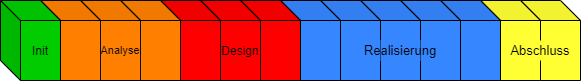
\includegraphics[scale=0.7]{\vorlagenOrdner/Bilder/Projektphasen}
			\end{center}
			\caption{Zeitplanung}
		\end{figure}

	\subsection{Phasen/Iterationen}
	\minisec{Phasen}
		Wir halten uns an die folgenden 5 Phasen: 

		\begin{table}[!h]
			\begin{tabularx}{\textwidth}{lll}
				\toprule
				Farbe* & Bezeichnung & Zeitrahmen \\
				\midrule
				\textcolor{green}{Grün} & Initialisierung & 1 Woche \\
				\textcolor{orange}{Orange} & Analyse & 3 Wochen \\
				\textcolor{red}{Rot} & Design & 3 Wochen \\
				\textcolor{blue}{Blau} & Realisierung & 6 Wochen \\
				\textcolor{yellow}{Gelb} & Abschluss & 2 Wochen \\
				\bottomrule
			\end{tabularx}
			\caption{Projektphasen}
		\end{table}

		\minisec{Iterationen}
		Die Iterationen werden wöchentlich durchgeführt.
		Da wir auch ein Mal in der Woche das Meeting haben passt das gut aufeinander.

		\begin{table}[!h]
			\begin{tabularx}{\textwidth}{lXll}
				\toprule
				Iteration & Inhalt & Start & Ende \\
				\midrule
				Initialisierung & Projektstart und Kick-Off Meeting & 20.02.2020 & 23.02.2020 \\
				Analyse 1 & Projektplanung & 24.02.2020 & 01.03.2020 \\
				Analyse 2 & Evaluation Module (Nornir, Napalm, Openconnect) & 02.03.2020 & 08.03.2020 \\
				Analyse 3 & Requirements \& Analyse Testcases & 09.03.2020 & 15.03.2020 \\
				Design 1 & Architekturdesign & 16.03.2020 & 22.03.2020 \\
				Design 2 & Testen der Module & 23.03.2020 & 29.03.2020 \\
				Design 3 & Prototyp programmieren & 30.03.2020 & 05.04.2020 \\
				Realisierung 1 & [Placeholder] & 06.04.2020 & 12.04.2020 \\
				Realisierung 2 & [Placeholder] & 13.04.2020 & 19.04.2020 \\
				Realisierung 3 & [Placeholder] & 20.04.2020 & 26.04.2020 \\
				Realisierung 4 & [Placeholder] & 27.04.2020 & 03.05.2020 \\
				Realisierung 5 & [Placeholder] & 04.05.2020 & 10.05.2020 \\
				Realisierung 6 & Fertigstellung und Refactoring & 11.05.2020 & 19.05.2020 \\
				Abschluss 1 & Bugfixes, Refactoring und Dokumentation & 08.05.2020 & 19.05.2020\\
				Abschluss 2 & Fertigstellung Schlussbericht & 20.05.2020 & 28.04.2020\\
				\bottomrule
			\end{tabularx}
			\caption{Projektiterationen}
		\end{table}

	\subsection{Meilensteine}
	Im Projekt wurden folgende Meilensteine festgelegt.
		\begin{table}[!h]	
			\begin{tabularx}{0.9\linewidth}{lllX}
				\toprule
				Nr & Bezeichnung & Termin & Beschreibung \\
				\midrule
				M1 & Projektplan & So 01.03.2020 & Grundentwurf der Requirements, Risikoanalyse \& -management, Projektorganisation, Managementabläufe, Infrastrukturentwurf, Qualitätsmassnahmen Grundentwurf.\\
				\midrule
				M2 & Requirements & So 15.03.2020 & Ausgearbeitete Requirements, Nichtfunktionale Anforderung, Zu verwendende Tools und Schnittstellen beschrieben.\\
				\midrule 
				M3 & Prototyp & So 05.04.2020 & Architektur festgeleg, Schnittstellen angelegt, Architekturdokumentation, Testprozeduren eingerichtet und UnitTests erstellt, Erster lauffähiger Prototyp.\\
				\midrule
				M4 & Feature Freeze & Do 07.05.2020 & Hauptfunktionalität der Software implementiert, Bugs sind bekannt und Dokumentiert, Codedokumentation zu 60\% fertiggestellt.\\
				\midrule
				M5 & Codefreeze \& Codeabgabe & Di 19.05.2020 & Bugfixes erstellt, Tests sind alle erfolgreich, Codedokumentation zu 60\% fertiggestellt.\\
				\midrule
				M6 & Projektabgabe & Do 28.05.2020 & Dokumentation fertiggestellt und abgegeben.\\
				\bottomrule
			\end{tabularx}
		\caption{Meilensteine}
		\end{table}	

	\subsection{Besprechungen/Protokolle}
	\label{sec:dates}
		Es wurden zwei Termine vereinbart, an welchen sich die Projektmitglieder treffen. 
		Bei beiden Terminen stehen jeweils mindestens 6 Lektionen zur Verfügung.

		\begin{table}[!h]
			\begin{tabularx}{0.9 \linewidth}{llX}
				\toprule
				Nr & Wann & Beschreibung \\
				\midrule
				1 & Dienstag 10:00 - 17:00 & Gemeinsame Arbeit der Projektmitglieder \\
				2 & Donnerstag 08:00 - 17:00 & Gemeinsame Arbeit der Projektmitglieder \\
				3 & Donnerstag 14:00 - 15:00 & Besprechung mit Projektbetreuern \\
				4 & Samstag 14.03.2020 & Dokumentation und Risikoreduktion\\
				5 & Samstag 28.03.2020 & Dokumentation und Risikoreduktion\\
				6 & Samstag 11.04.2020 & Dokumentation und Risikoreduktion\\
				7 & Samstag 25.04.2020 & Dokumentation und Risikoreduktion\\
				8 & Samstag 09.05.2020 & Dokumentation und Risikoreduktion\\
				9 & Samstag 23.05.2020 & Dokumentation und Risikoreduktion\\

				\bottomrule
			\end{tabularx}
			\caption{Termine}
		\end{table}
			

\section{Risikomanagement}
\label{sec:risikomanagement}

	\subsection{Risiken}
		Eine Riskoanalyse mit gewichtetem Schaden und Informationen zur Vorbeugung ist auf der Ablage zu
		finden (siehe Dokument TechnischeRisiken.xlsx)

	\subsection{Umgang mit Risiken}
		Um Probleme gerade während der Init/Analyse Phase möglichst früh zu erkennen, 
		arbeiten wir wöchentlich zwei Tage nebeneinander, um uns über mögliche Probleme auszutauschen. 
		Desweiteren suchen wir auch den Kontakt zum Betreuer sobald Unklarheiten im Team herrschen.
		Einmal alle zwei Wochen treffen wir uns am Samstag für drei bis vier Stunden, um an der Dokumentation und and der Reduktion aufgetretener Risiken zu arbeiten. Die genauen Termine werden im Kapitel~\ref{sec:dates} beschrieben.

\section{Infrastruktur}
	Alle Arbeiten zum Projekt werden von den Projektmitgliedern auf Ihrem jeweiligen Laptop verrichtet.
	Alternativ stehen in den Studienarbeitszimmern Computer zur Verfügung, mit denen im falle eines Geräteausfalls weitergearbeitet werden kann.
	Für das Testen der Software wird vom Institut für Networked Solutions eine Routerinfrastruktur zur Verfügung gestellt.
	Die genauen Ausmasse der Infrastruktur sind zum Zeitpunkt der Erstellung des Projektplans noch nicht spezifiziert.
	

	\subsection{Übersicht der Tools}
		Für die Umsetzung des Projektes werden folgende Tools verwendet: \\[2ex]
		\begin{table}[!h]
			\begin{tabularx}{0.9\linewidth}{lX}
				\toprule
				Bezeichung & Beschreibung \\
				\midrule
				Git & Versionsverwaltung \\
				PyCharm & Entwicklungsumgebung \\
				Visual Studio Code & Editor für die Dokumentation\\
				\bottomrule
			\end{tabularx}
		\caption{Tools im Projekt}
		\end{table}
		
		

\section{Qualitätsmassnahmen}
	\subsection{Allgemein}

	\subsection{Testing}
		Für das Unti-Testing wird das Python-Modul PyTest verwendet, ein Framework, welches das einfache Testen von Pythoncode erlaubt.

	\subsection{Besprechungen}

	\subsection{Versionskontrolle}
		Sämtliche Dokumente werden in einem Git Repository abgelegt. Damit wird, dank der Versionskontrolle, 
		jede Änderung nachvollziehbar und es können auf sämtlichen alten Versionen zugegriffen werden.

	\subsection{Dokumente}

	\subsection{Code-Qualität}
		Um die Codequalität zu gewährleisten, werden folgende Massnahmen ergriffen:
		\begin{itemize}
			\item Unittests, um Fehler im Code zu verhindern oder früh zu finden.
			\item In der Versionsverwaltung wird mit Feature-Branches gearbeitet, damit Änderungen nicht zu Merge-Konflikten führen.
			\item Merges in den Development-Branch dürfen nur nach einem erfolgreichen Pull-Request durchgeführt werden.
			\item Pull-Requests werden vom jewils anderen Teammitglied überprüft und allfällige Probleme müssen vor der Annahme korrigiert werden.
			\item Im Git wird ein CI/CD (Continous Integration/Continous Delivery) aufgesetzt, das bei Änderungen im Development-Branch Tests durchführt.
			\item Getestet wird die einhaltung der Coderichtlinien, Vorherig definierte Tests und das erfolgreiche durchlaufen des Build-Prozesses.
			\item Bekannte Bugs werden mittels Git Issues erfasst und verwaltet. Das Abarbeiten dieser Issues ist teil des Projekts und beim Meilenstein M5:Codefreeze \& -abgabe sollten sich keine Issues mehr auf dem Repository befinden
		\end{itemize}
\end{document}